\section{Concepts}

\subsection{Operating Systems}

\begin{frame}{IT trends}
	\begin{itemize}
		\item more resources
			\begin{itemize}
			\item better hardware at lower costs
			\item higher standards for software quality
			\end{itemize}
		\item more users
			\begin{itemize}
			\item accesibility at an earlier age
			\item shared access to the same device
			\end{itemize}
		\item data consolidation
			\begin{itemize}
			\item data warehousing
			\item service unification
			\item separate access policies
			\end{itemize}
		\item increased flexibility
			\begin{itemize}
			\item differentiated access
			\item straighforward configuration
			\item focus on usability
		\end{itemize}
	\end{itemize}
\end{frame}

\begin{frame}{OS Recap}
	\begin{columns}[T]
		\begin{column}{.5\textwidth}
			\begin{itemize}
			\item Resources
				\begin{itemize}
				\item CPU
				\item memory
				\item peripherals
				\end{itemize}
			\item Structures
				\begin{itemize}
				\item the Scheduler
				\item the Pager
				\item Filesystems
				\end{itemize}
			\item the Kernel
				\begin{itemize}
				\item handles hardware
				\item exposes capabilities
				\item manages resources
				\end{itemize}
			\end{itemize}
		\end{column}
		\begin{column}{.5\textwidth}
			\begin{figure}[ht]
				\vspace*{-0.7cm}
				\caption{The Memory Pager}
				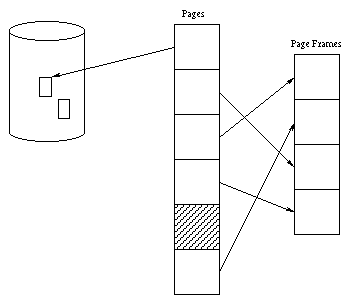
\includegraphics[height=0.3\textheight]{img/pager.png}
			\end{figure}
			\begin{figure}[ht]
				\vspace*{-0.7cm}
				\caption{The Scheduler}
				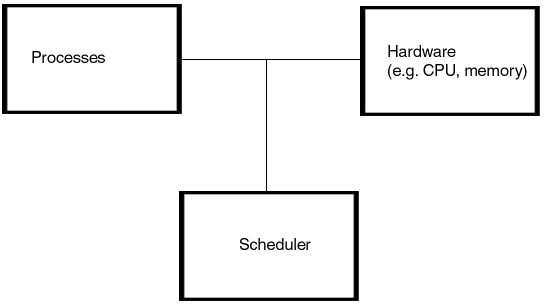
\includegraphics[height=0.3\textheight]{img/scheduler.png}
			\end{figure}
		\end{column}
	\end{columns}
\end{frame}

\subsection{Virtualization}

\begin{frame}{Virtualization}
	\begin{columns}[T]
		\begin{column}{.5\textwidth}
			\begin{itemize}
			\item Key aspects:
				\begin{itemize}
				\item simulation of software and/or hardware
				\item virtual machines
				\item autonomous computing
				\item utility computing
				\end{itemize}
			\item Advantages:
				\begin{itemize}
				\item better resource usage
				\item lower running costs
				\item application sandboxing
				\end{itemize}
			\item Concerns:
				\begin{itemize}
				\item management
				\item isolation
				\item performance
				\item applicability
				\end{itemize}
			\end{itemize}	
		\end{column}
		\begin{column}{.5\textwidth}
			\begin{figure}[hb]
				\centering
				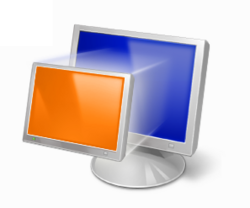
\includegraphics[width=\textwidth]{img/virt.png}
			\end{figure}
		\end{column}
	\end{columns}
\end{frame}

\begin{frame}{OS-level Virtualization}
	\begin{itemize}
	\item one host
	\item multiple running OS instances
	\item rootfs, system libs, binaries
	\end{itemize}
	
	OS instance = a process hierarchy
	
	OS level virtualization = \textbf{partitioning} the process tree
	
	Advantage: \textbf{close to 0\% performance overhead}
	
	Flaw: \textbf{shared kernel}
\end{frame}